%%%%%%%%%%%%%%%%%%%%%%%%%%%%%%%%%%%%%%%%%%%%%%%%%%%%%%%%%%%%%%%%%%%%%%%%%%%%%%%
%                                                                             %
%           LATEX TEMPLATE FOR THESIS                                         %
%           ______________                                                    %
%                                                                             %
%           Last revision: April 11, 2025                                     %
%                                                                             %
%%%%%%%%%%%%%%%%%%%%%%%%%%%%%%%%%%%%%%%%%%%%%%%%%%%%%%%%%%%%%%%%%%%%%%%%%%%%%%%
% Use the 'twoside' option if you want to print double-sided. E.g.:
% \documentclass[twoside,12pt]{report}
% It is recommended to decrease font size for PhD theses in 17x24 format. E.g.:
% \documentclass[11pt]{report}
\documentclass[12pt]{report}

% --- PREAMBLE ---------------------------------------------------------------
% Insert here any packages to include or custom command definitions

% Language Selection
% CHANGED: Switched from 'italian' to 'english'
\usepackage[english]{babel}

\usepackage{tesi}

% --- ADD THESE LINES HERE ---
\usepackage{float}
\usepackage{longtable}
\usepackage{booktabs}   
\usepackage{tabularx}   
\usepackage[edges]{forest} 
\usepackage{graphicx}
\usepackage{xcolor}
\usepackage{tikz} % TikZ must be loaded first
\usetikzlibrary{positioning, shadows, calc, fit, backgrounds, arrows.meta, decorations.pathreplacing} % Then load the libraries
% --- Where to look for figure files (upload the diagram PDFs into a "figures/" folder) ---
\graphicspath{{figures/}{immagini/}{./}}
% ----------------------------

% You can use the default LaTeX font with the relative package option
% \usepackage[defaultfont]{tesi}
% There is also an option for the 17x24 format for PhD theses
% \usepackage[phd]{tesi}

% If copy-pasting from the generated PDF loses spaces,
% try uncommenting the following line
% \pdfinterwordspaceon

% !!! THESIS INFORMATION TO FILL IN !!!

%   UNIVERSITY AND DEGREE COURSE:
\university{University of Milan}
\unilogo{immagini/loghi/unimi}
\faculty{Faculty of Science and Technology}
\department{Department of Computer Science\\Giovanni Degli Antoni}

% Adjust the specific degree name below:
% For Master's: "Master's Degree in..."
% For Bachelor's: "Bachelor's Degree in..."
\cdl{Master's Degree in\\Computer Science}

%   THESIS TITLE:
\title{Self-Supervised Learning for Music Information Retrieval: State of the Art and Applications}
% This command (optional) overwrites \title for the cover page
% Can be used to print special characters while keeping metadata clean
\printedtitle{Self-Supervised Learning for Music Information Retrieval:\\State of the Art and Applications}

%   AUTHOR:
\author{Arvin [Your Surname]}
\matricola{123456}

%   TYPE OF THESIS:
% "Bachelor's Project" (or "Elaborato Finale") for Bachelor's degrees
% "Master's Thesis" (or "Tesi di Laurea") for Master's degrees
\typeofthesis{Master's Thesis}

%   SUPERVISOR AND CO-SUPERVISOR:
% Note: 'Relatore' = Supervisor, 'Correlatore' = Co-supervisor
\relatore{Prof. Giovanni Degli Antoni}
\correlatore{Prof. Brian W. Kernighan}
% \correlatore{Prof. Dennis M. Ritchie} % Uncomment if you have a second co-supervisor

%   LABORATORY:
% This section creates a closing page with the logo of the entity/lab
% where the internship took place.
% Below are the predefined labs for the department:
% \adaptlab
% \aislab
% \anacletolab
% \bisplab
% \connetslab
% \everywarelab
% \falselab
% \iebilab
% \islab
% \lailalab
% \lalalab
% \lawlab
% \laserlab
 \limlab
% \mipslab
% \optlab
% \phuselab
% \ponglab
% \sesarlab
% \spdplab

% Example of closing page customization
% (comment out if one of the macros above is sufficient)
% \lab{Research Laboratory}
% \lab[in collaboration with]{Company Name}
% \laburl{https://di.unimi.it/it/ricerca/risorse-e-luoghi-della-ricerca/laboratori-di-ricerca}
% \lablogo{immagini/redqmark}

% With this command, you can change the size (max height and width) of logos
% \setlength\lablogosize{25mm}

%   ACADEMIC YEAR
% \the\year inserts the current year.
% Do NOT insert in 2024-2025 format, but insert only 2024
% (The template likely auto-formats it to "2024/2025")
\academicyear{\the\year} 

%   INDICES/TABLES:
% List of figures (optional)
% \figurespagetrue
% List of tables (optional)
% \tablespagetrue
% Preface in Table of Contents (optional)
\prefaceintoctrue
% Table of Contents in Table of Contents (optional)
\tocintoctrue
% --- END PREAMBLE ----------------------------------------------------------
\begin{document}

% Automatic cover generation
% Centers the cover on the sheet: use this command for the external cover
% \makecenteredfrontpage
% Cover aligned with other pages: use this command for the internal cover
\makefrontpage

% 
%			DEDICATION AND/OR QUOTE PAGE
%			Optional, this is the only thing you have to format manually
%

{\raggedleft \large \sl This work is dedicated to my parents\\
	
	\vspace{2cm}
	
	``What I cannot create, I do not understand''
	
	\bigskip
	
	\--- Richard Feynman\\
  
	\vspace{2cm}
	
	``It's not only powerful,\\but it's also inadequate''
	
	\bigskip
	
	\--- Miller Puckette\\}

\clearpage
\beforepreface

% 
%			PREFACE (Optional)
%

% \prefacesection{Preface}
% Prefaces are not very common; however, sometimes one may wish to say something that falls outside the work itself (like a meta-comment on the thesis), or provide information regarding the project within which the thesis is situated (in this case, it is likely the supervisor writing this part).

%
%			ACKNOWLEDGMENTS (Optional)
%

\prefacesection{Acknowledgments}
This section, which is optional, contains your acknowledgments.

%
%			Automatic Table of Contents generation
%

\afterpreface

% 
%			CHAPTER 1: Introduction or Abstract
% 

\chapter{Introduction}
\label{ch:introduction}

This document serves a dual purpose: on one hand, it shows a complete example of a thesis written in \LaTeX\ and compliant with the PDF/A standard; on the other, it contains suggestions and answers to frequently asked questions by students. Therefore, a careful reading is recommended.

\section{The Template}
If this document was obtained via direct file sharing, it is advisable to access the continuously updated version available on Overleaf. 
\begin{center}
    \url{https://www.overleaf.com/read/hmffzxzhhdqn}
\end{center}

This template has been developed over the years by members of the Laboratory of Music Informatics (LIM) at the University of Milan, specifically by: Giorgio Presti, Luca Andrea Ludovico, Federico Avanzini, and Marco Tiraboschi.

It was primarily intended for final projects of the Bachelor's Degree in Music Informatics, and later extended to other degree courses of the Department of Computer Science, but it can be adapted for other courses by changing the metadata in the preamble. In the rest of the document, where not specified, we will use the term \textit{thesis} in its generic sense, which includes Bachelor's final projects.

\section{Content}
\label{sec:content}

Sometimes, theses can have strong interdisciplinary connotations. However, it is fundamental to remember that these are works in the field of computer science, and this aspect must emerge clearly. Even projects with more humanistic content must show scientific rigor and an effort toward formalization. Concretely, diagrams, tables, graphical and/or mathematical formalisms, and significant portions of code (where possible) are highly appreciated.

A written work of this extent always starts from a prior point, typically the analysis of the state of the art and literature. A personal contribution is then required (and original, in the case of Master's theses) to reach a conclusion formulated by the author, potentially even in contrast with current thought or with what was intended at the beginning of the work.

Three phases must emerge clearly:
\begin{itemize}
	\item analysis of the state of the art and/or literature;
	\item personal contribution to the research;
	\item conclusions reached, and potential future developments.
\end{itemize}

Taken together, these three components must make the {\em relevance} of the work evident, in terms of:
\begin{itemize}
\item clarity in defining the problem, motivations, and objectives of the thesis; 
\item connection with the literature (to show that the topic of the thesis is of interest to the scientific community);
\item relevance of the topic within the scope of computer science disciplines.
\end{itemize}


\section{Thesis Organization}
\label{sec:organization}

The choice of how to structure an extended work, such as a final project or a thesis, is neither simple nor unique; therefore, the points listed below should be taken as generic suggestions and adapted to one's personal situation.

\begin{figure}[t]
	\centering
	\includegraphics[width = \textwidth, trim={0 25mm 0 0}, clip]{immagini/ideas2text.png}
	\caption{The process of transforming ideas into text~\cite{hamalainen2019web}.}
	\label{fig:ideas2text}
\end{figure}
Before starting to write text, it is fundamental to create a hierarchically organized table of contents (thesis, chapters, sections, subsections, etc.). Once a satisfactory index is obtained, it can be filled with the text of the thesis. 
A computer science approach to the issue is the following: writing a thesis means starting from a graph of ideas~\cite{hamalainen2019web} and arriving at creating a tree of textual content (a \textit{minimum spanning tree} of the idea graph!). The tree represents the text structure, where the root node is the thesis itself, its children are the chapters, etc. The leaves of the tree represent the finest-level subsections.  
%
Ideally, the content tree should have the following characteristics:
\begin{itemize}
\item be balanced;
\item have a height $h=4$ or $5$; 
\item be an $n$-ary tree with $2\leq n \leq 7$
\end{itemize}
The textual content of all nodes at the same level of the tree should also be as balanced as possible (for example, it would be wrong to have one chapter of one page and another of $30$ pages).
% Chapters into which the work is divided should tend to occupy a homogeneous number of pages. 
An imbalance in favor of the chapter describing one's specific work and innovative contributions is tolerated.

Limited to the second level of the tree (chapters), a purely indicative example of an outline for an experimental thesis is as follows:
\begin{itemize}
    \item Table of Contents
    \item Introduction
    \item State of the Art Chapter
    \item Chapter on technologies used\footnote{This chapter can be omitted if the only technologies used are standard tools like Python, JavaScript, C++, Matlab, etc.}
    \item Chapter on the case study or software implemented
    \item Chapter on tests performed
    \item Brief chapter on conclusions and future developments
    \item Bibliography and potential Webography
    \item Appendices, if any (e.g., complete code listings, user manual, proofs, etc.)
\end{itemize}
It will therefore be appropriate to include, in the introductory chapter, an explicit reference to the document structure. For example: ``The present work is organized as follows: in Chapter 1 \dots''.



\section{Style and Form}
\label{sec:form}


The style of a scientific thesis must be exact, clear, compact, and objective~\cite{strunk1999style}.

{\em Exact} means that every word used signifies only what it is intended to express. It is appropriate to try to avoid synonyms when referring to important concepts. Where possible, variables should be defined (frequency $f$, time $n$, etc.) and used systematically. Vague and non-quantitative expressions (``quite large'', ``practically all'', ``very few'', \ldots) should be avoided as much as possible. Use pronouns sparingly; it is better to repeat a noun in the text rather than leaving ambiguities.

{\em Clear} means that structure and form must be functional in transmitting information in the most immediate and understandable way. Chapter and section titles must be illustrative of the contents (it is also useful to have brief text at the beginning of a chapter or section before moving to subsections). The text must be logically divided into sentences, paragraphs, and blocks: short, direct, and declarative paragraphs are preferable, limiting subordinate clauses and parentheticals, and blocks must be consistent with the logic of the discourse. The use of technical terms should be limited only to necessary cases. Acronyms must also be used sparingly and explained the first time they are used. 

{\em Compact} means one must write only what is necessary. Repetitions of concepts and observations must be avoided. Descriptions and details not necessary for understanding the general discourse must be limited. In particular, trivial observations that are obvious to the reader should be avoided. Between a verbose form (``in consideration of the fact that\ldots'') and a more synthetic equivalent (``because\ldots''), the latter is preferred.

{\em Objective} means that what is written must be devoid of subjective elements and elements that might influence evaluation. Personal considerations (``I first came up with this idea during\ldots'') must be carefully avoided, as well as debatable statements whose judgment is left to the author's personal opinion. The only way to support such stances is to provide scientific data proving one's thesis, or to refer explicitly to a bibliographic antecedent (``ipse dixit'') citing its source in the bibliography. Finally, the manuscript must be written in an impersonal form. Sentences such as ``During my experience, I deepened the themes\dots'' are easily replaceable with phrases such as ``During the analysis phase, the themes of\dots were investigated''.

Appropriate use of figures and tables is essential to support the points just discussed. Figures and tables must have self-explanatory captions (which do not require reading the main text to understand their meaning). However, the main text must always contain a reference to the figure or table (``As shown in Fig.1, \ldots''). The use of graphical diagrams (an audio processing algorithm block diagram, a software project conceptual schema, etc.) is particularly useful to support the clarity and compactness of the exposition.
% 
%			CHAPTER 2: State of the Art
% 

\chapter{State of the Art}
\label{chap:state_of_the_art}

\section{Introduction}
Music Information Retrieval (MIR) aims to help computers understand and organize musical content, supporting tasks such as genre tagging, instrument detection, beat tracking, and emotion analysis. Many MIR systems still rely on large labeled datasets, which are costly to create and often subjective—especially for emotion and perceptual similarity.

Self-Supervised Learning (SSL) has recently become a strong alternative, allowing models to learn useful audio representations from unlabeled music. Methods like CLMR, BYOL-A, MERT, and AudioMAE show that SSL features can match or outperform supervised models on tagging and classification. However, most work focuses on broad tasks, while perceptual and affective aspects of music remain less explored.

Two areas with clear gaps are Music Emotion Recognition (MER) and Music Similarity Learning. Emotion datasets such as DEAM and EMO-Music are small and subjective, and similarity is often approximated with genre or metadata rather than human perception. Existing systems also struggle to explain why two tracks are considered similar.

This thesis investigates modern SSL models—contrastive, predictive, and masked—for emotion recognition and similarity learning under low-label settings. It also explores a simple RAG-inspired retrieval step to provide clear, metadata-based explanations. The goal is to evaluate how SSL can improve emotion modeling, perceptual similarity, and transparency in MIR applications.

\section{Self-Supervised Learning for Audio}
\begin{figure}[H]
\centering
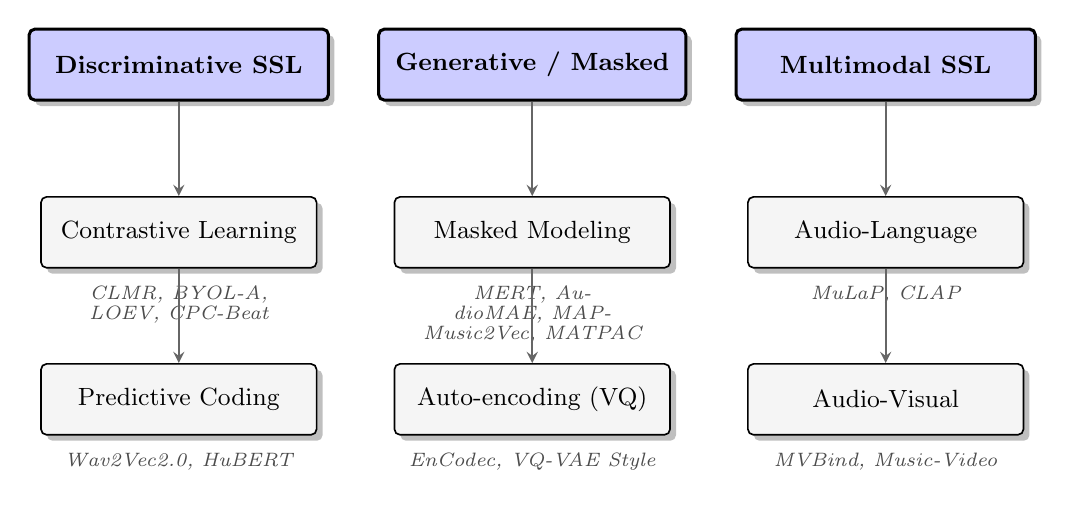
\begin{tikzpicture}[
    node distance=1.2cm and 0.4cm, % Increased vertical and horizontal spacing
    box/.style={
        draw, 
        rounded corners=2pt, 
        align=center, 
        fill=white, 
        font=\small, 
        drop shadow, 
        line width=0.6pt,
        minimum height=0.9cm,
        inner sep=6pt % Padding inside the boxes
    },
    cat/.style={box, fill=blue!20, line width=1.1pt, minimum width=3.8cm},
    subcat/.style={box, fill=gray!8, minimum width=3.5cm},
    paper/.style={font=\scriptsize\itshape, text=black!70, align=center, execute at begin node=\setlength{\baselineskip}{1.2ex}}
]

% Paradigms (Level 1)
\node[cat] (discriminative) {\textbf{Discriminative SSL}};
\node[cat, right=0.6cm of discriminative] (generative) {\textbf{Generative / Masked}};
\node[cat, right=0.6cm of generative] (multimodal) {\textbf{Multimodal SSL}};

% Subcategories (Level 2) - Positioned relative to Level 1
\node[subcat, below=of discriminative] (contrastive) {Contrastive Learning};
\node[subcat, below=1.2cm of contrastive] (predictive) {Predictive Coding};

\node[subcat, below=of generative] (masked) {Masked Modeling};
\node[subcat, below=1.2cm of masked] (vae) {Auto-encoding (VQ)};

\node[subcat, below=of multimodal] (lang) {Audio-Language};
\node[subcat, below=1.2cm of lang] (vision) {Audio-Visual};

% Papers (Level 3) - Using "text width" to prevent horizontal spilling
\node[paper, below=0.1cm of contrastive, text width=3.3cm] (p1) {CLMR, BYOL-A, LOEV, CPC-Beat};
\node[paper, below=0.1cm of predictive, text width=3.3cm] (p2) {Wav2Vec2.0, HuBERT};
\node[paper, below=0.1cm of masked, text width=3.3cm] (p3) {MERT, AudioMAE, MAP-Music2Vec, MATPAC};
\node[paper, below=0.1cm of vae] (p4) {EnCodec, VQ-VAE Style};
\node[paper, below=0.1cm of lang, text width=3.3cm] (p5) {MuLaP, CLAP};
\node[paper, below=0.1cm of vision, text width=3.3cm] (p6) {MVBind, Music-Video};

% Connecting Arrows with a cleaner style
\draw[-stealth, thick, color=black!60] (discriminative) -- (contrastive);
\draw[-stealth, thick, color=black!60] (contrastive) -- (predictive);
\draw[-stealth, thick, color=black!60] (generative) -- (masked);
\draw[-stealth, thick, color=black!60] (masked) -- (vae);
\draw[-stealth, thick, color=black!60] (multimodal) -- (lang);
\draw[-stealth, thick, color=black!60] (lang) -- (vision);

\end{tikzpicture}
\caption{Modular architecture of SSL paradigms for MIR. This view categorizes frameworks by their objective function and primary model examples.}
\label{fig:modular_taxonomy}
\end{figure}

% \begin{figure}[ht]
% \centering
% \begin{forest}
%   for tree={
%     draw,
%     rounded corners,
%     node options={align=center},
%     edge={->},
%     l sep=0.8cm,
%     s sep=0.4cm,
%     fill=gray!5
%   }
%   [SSL in MIR
%     [Contrastive
%       [CLMR]
%       [BYOL-A]
%     ]
%     [Predictive / Masked
%       [MERT]
%       [AudioMAE]
%       [MATPAC++]
%     ]
%     [Cross-Modal
%       [MuLaP]
%     ]
%   ]
% \end{forest}
% \caption{Taxonomy of Self-Supervised Learning model families for MIR.}
% \label{fig:ssl_taxonomy}
% \end{figure}



\subsection{Contrastive Learning}
Contrastive learning has become one of the most influential families of self-supervised approaches for music audio representation. The main idea is to learn embeddings that place different augmented versions of the same audio close together, while pushing unrelated audio apart in the embedding space. Early work, such as CLMR \cite{spijkervet_contrastive_2021} adapted the SimCLR framework to raw music waveforms and demonstrated that contrastive pre-training can match or surpass supervised baselines on tagging datasets such as MagnaTagATune and the Million Song Dataset using only a linear classifier. Later studies confirmed that contrastive objectives remain highly competitive across large-scale music tagging tasks. For example, a large benchmark on multi-view self-supervision \cite{meseguer-brocal_experimental_2024} showed that contrastive methods consistently outperform BYOL-style, clustering-based, and VICReg-style alternatives when trained on millions of unlabeled tracks.

Beyond tagging, contrastive learning has been applied to more specialized MIR tasks. Several works explore rhythm-sensitive representations by contrasting tempo- and structure-preserving augmentations. A few-shot contrastive beat-tracking framework \cite{gagnere_contrastive_2024} learns tempo-invariant rhythmic features, enabling rapid domain adaptation with very limited labeled data. Similarly, Zero-Note Samba \cite{desblancs_zero-note_2023} demonstrated that contrasting time-domain rhythm augmentations can achieve near-supervised performance on beat-tracking benchmarks.

A key limitation of classical contrastive learning is its tendency to enforce excessive invariance—e.g., removing tempo, pitch, or timbre cues that are musically meaningful. Recent work attempts to address this. The LOEV and LOEV++ frameworks \cite{guinot_leave-one-equivariant_2025} preserve transformation-specific information by assigning dedicated latent subspaces for pitch, tempo, and other augmentations, improving key estimation, tempo prediction, and music retrieval while maintaining strong tagging accuracy.

Contrastive learning has also been used in perceptual similarity and large-scale retrieval applications. Triplet-based CNN models \cite{thome_musical_2022} and neural audio fingerprints \cite{chang_neural_2021} rely on contrastive objectives to learn robust embeddings for real-world music search, achieving strong performance under noisy or transformed audio conditions. Other works extend the paradigm to cross-modal retrieval. Audio–sheet-music alignment \cite{carvalho_self-supervised_2023} and cross-modal video–music recommendation systems \cite{teng_mvbind_2024,stewart_semi-supervised_2025,pretet_cross-modal_2021} learn joint spaces where audio clips are pulled toward corresponding symbolic or visual representations. These models show that contrastive supervision can generalize across modalities when consistent cues (e.g., rhythm, mood, or harmonic structure) are shared.

Finally, contrastive learning continues to be an important baseline for hybrid or semi-supervised scenarios. SemiSupCon \cite{guinot_semi-supervised_2024} combines supervised and contrastive losses, improving tagging and emotion recognition when only a small portion of data is labeled. Studies analyzing augmentation strategies \cite{choi_towards_2022} emphasize that the choice of pitch shifts, time-stretching, filtering, or reverb plays a critical role in downstream performance. Overall, contrastive learning remains one of the most stable and transferable SSL families in MIR, consistently delivering strong results across tagging, rhythm analysis, retrieval, cross-modal alignment, and low-label scenarios.

\subsection{Predictive Coding Approaches}
Predictive self-supervised learning focuses on forecasting or reconstructing masked audio, enabling models to learn musical structure without labels. Large music-focused models such as MERT \cite{li_mert_2024}
use predictive objectives on massive unlabeled corpora to capture long-term patterns, timbre, and harmony, achieving strong results in tagging and key or chord estimation. Other studies examine whether speech-based SSL models like wav2vec2.0 or HuBERT can transfer to music \cite{ma_effectiveness_2023}
showing good low-level feature transfer but limited understanding of higher-level musical semantics. Predictive features have also been applied to singing voice conversion \cite{chen_singing_2025}
where melody-sensitive SSL representations allow systems to change vocal timbre while preserving pitch and rhythm, even in mixed audio. Overall, predictive coding offers strong temporal modeling and remains an effective alternative when tasks rely on melody, structure, or long-range dependencies.

\subsection{Masked Modeling Approaches}

Masked modelling is a powerful self-supervised paradigm adapted from NLP for Music Information Retrieval (MIR), where models are trained to reconstruct randomly masked segments of input data to learn meaningful contextual representations.

Large-scale masked modelling frameworks, such as foundation models trained on extensive music datasets, utilize transformer encoders to reconstruct masked spectrogram patches, setting new benchmarks for Masked Autoencoder (MAE)-style SSL across tagging, beat tracking, and key estimation tasks \cite{won_foundation_2024}. Simpler approaches like MAP-Music2Vec achieve competitive results through a lightweight masked prediction of mel-spectrogram patches, demonstrating the effectiveness of the basic principle for tasks like tagging and emotion recognition \cite{li_map-music2vec_2022}. Further enhancing this, the MATPAC framework combines masked latent prediction with classification of high-level acoustic attributes to improve both fine-grained and global understanding for downstream tasks \cite{quelennec_matpac_2025}.

Innovations extend the masking technique to more complex inputs, such as the SSLAM framework, which trains on mixtures of multiple sound sources. By reconstructing masked segments in mixed audio, the model learns to separate and represent overlapping components, enhancing music tagging and separation performance \cite{alex_sslam_2025}. The utility of masked modelling also bridges representation learning and generation; for instance, AudioLDM 2 integrates masked audio modelling with latent diffusion for controllable, high-fidelity sound generation \cite{liu_audioldm_2024}. Furthermore, the paradigm is effective in symbolic MIR, where a masked-sequence transformer can predict missing harmonic information to produce musically coherent harmonizations \cite{rhyu_translating_2022}.


\subsection{Multimodal and Cross-Modal SSL}


The integration of **multimodal signals**, specifically music audio and descriptive text, is driving the development of semantically rich self-supervised representations in MIR. A prominent example is MuLaP, which learns music audio representations via weak language supervision \cite{manco_learning_2022}. MuLaP employs a multimodal pre-training framework that jointly trains audio and text branches using masked modeling and an audio-text matching task. This approach successfully captures cross-modal structure, yielding audio embeddings that significantly improve performance on diverse downstream tasks like tagging, genre, and emotion recognition.

\subsection{Task-Specific and Hybrid SSL Approaches}


A significant body of work focuses on adapting and specializing general self-supervised learning (SSL) models for specific MIR tasks, demonstrating their remarkable transferability and generalization capabilities.

Several studies highlight the transfer of pre-trained embeddings to rhythm and tempo analysis. Pitch-based SSL models like MERT and wav2vec2 have been successfully adapted for tempo estimation, proving that pitch-oriented features also encode rhythmic cues \cite{gagnere_adapting_2024}. A fully self-supervised approach even reframed tempo estimation as a binary classification problem—determining if two tracks share the same tempo—achieving competitive results without any labeled data \cite{henkel_tempo_2024}. More generally, pre-trained embeddings such as OpenL3 have been shown to provide robust, transferable representations that outperform supervised baselines for various audio classification tasks, especially when labeled data is scarce \cite{grollmisch_analyzing_2021}.

In advanced classification and analysis, MERT is frequently leveraged. MERTech fine-tunes MERT for instrument playing-technique detection by adding multi-task objectives for pitch and onset, yielding strong results by transferring knowledge from the large-scale pre-training \cite{li_mertech_2024}. MERT features are also central to new tasks, such as lead instrument detection in multitrack recordings, where a track-wise attention model with permutation augmentation significantly outperforms traditional baselines \cite{ou_lead_2025}. Further research confirms the strong transferability of SSL models (Wav2Vec2.0, WavLM, MERT) to automatic singing voice understanding tasks, often matching or surpassing supervised performance with limited training data \cite{yamamoto_toward_2023}.

To enhance interpretability and learning quality, hybrid methods are employed. PECMAE uses pre-trained SSL autoencoders (EnCodecMAE) to decouple feature learning from prototype training, creating a prototype-based interpretable model for classification that offers explainable, sonifiable prototypes \cite{alonso-jimenez_leveraging_2024}. For metric learning, integrating a self-supervised contrastive loss as an auxiliary objective alongside the supervised loss enhances both retrieval and auto-tagging performance without freezing the encoder \cite{akama_self-supervised_2023}.

Other specific applications include learning semantic similarity in symbolic music using self-supervised adversarial architectures \cite{bretan_learning_2019}, creating disentangled style and content representations for one-shot music style transfer using a self-supervised VQ-VAE \cite{cifka_self-supervised_2021}, and developing S-KEY, a self-supervised system for major/minor key classification that uses pseudo-labels to match supervised state-of-the-art results \cite{kong_s-key_2025}. Finally, the use of multi-task SSL pre-training by reconstructing hand-crafted features (e.g., MFCCs) demonstrates that re-weighted combinations of SSL objectives yield more general and transferable music embeddings \cite{wu_multi-task_2021}, while multi-view learning is used to explicitly disentangle shared and private information for interpretable, factorized audio representations \cite{wilkins_self-supervised_2024}.



\section{MIR Tasks and SSL Applications}

The emergence of self-supervised learning (SSL) has reshaped Music Information Retrieval (MIR) by enabling general-purpose feature learning from large collections of unlabeled music. Early studies focused on contrastive frameworks such as CLMR \cite{spijkervet_contrastive_2021} and BYOL-A \cite{niizumi_byol_2023}, while recent works extend to predictive, masked, and multimodal approaches like MERT \cite{li_mert_2024}, AudioMAE \cite{AudioMAE2022}, and MuLaP \cite{manco_learning_2022}. These models have been adapted across diverse MIR tasks, where genre and tagging benefit from high-level semantics, instrument recognition requires timbral detail, and sound-event detection relies on temporal precision. This section summarizes representative applications and highlights a persistent research gap in music emotion recognition and similarity learning.

\subsection{Genre and Tagging}
Genre classification and multilabel tagging serve as primary stress-tests for music SSL, requiring the extraction of broad, high-level semantics such as instrumentation and mood from short excerpts. Contrastive and masked objectives excel here by learning invariance to nuisances like loudness or minor pitch shifts while preserving tag-correlated cues. Foundational contrastive works such as CLMR \cite{spijkervet_contrastive_2021}, CLAR \cite{saeed_contrastive_2021}, and BYOL-A \cite{niizumi_byol_2023} demonstrated that SSL could achieve strong results with limited labeled data. More recent approaches have further optimized this efficiency; for instance, MAP-Music2Vec provides a robust masked prediction baseline \cite{li_map-music2vec_2022}, while comparisons of multi-view SSL frameworks highlight their robustness in low-label regimes \cite{meseguer-brocal_experimental_2024}. Large-scale predictive models like MERT continue to set benchmarks by capturing complex musical dependencies \cite{li_mert_2024}.

\subsection{Instrument Recognition}
Instrument recognition necessitates rich spectral representations that generalize across varying recording conditions and instruments unseen during training. Recent research has moved beyond clip-level labeling toward finer granularity, employing SSL backbones for tasks such as lead-instrument detection and playing-technique recognition. Multi-task pre-training has been shown to yield more generalizable embeddings for instrument classification compared to single-task baselines \cite{wu_multi-task_2021}. Specific adaptations include MERTech, which fine-tunes MERT for playing-technique detection \cite{li_mertech_2024}, and track-wise attention models for lead instrument detection in multitrack audio \cite{ou_lead_2025}. Furthermore, frameworks like PECMAE leverage pre-trained autoencoders to learn interpretable prototypes, enhancing the explainability of instrument classification systems \cite{alonso-jimenez_leveraging_2024}.

\subsection{Sound Event Detection}
Sound Event Detection (SED) demands temporal precision and robustness to polyphony. While general-purpose models like CLAR \cite{saeed_contrastive_2021} and BYOL-A \cite{niizumi_byol_2023} provide strong time-sensitive features, recent specialized architectures focus on handling overlapping sources. MATPAC employs a masked latent prediction objective to improve the separation of acoustic attributes \cite{quelennec_masked_2025}, and SSLAM introduces mixture-aware training to aid frame-level detection without relying on large labeled corpora \cite{alex_sslam_2025}. These methods demonstrate that masked-latent objectives significantly improve the model's ability to delineate event boundaries in complex auditory scenes.

\subsection{Gap: Emotion Recognition and Similarity Learning}
Despite these advancements, Music Emotion Recognition (MER) and human-aligned similarity remain underexplored in SSL literature. MER faces challenges regarding subjective labels and temporal dynamics, while similarity is often treated as a proxy for genre rather than perceptual closeness. Existing efforts include triplet-based SSL for industrial search \cite{thome_musical_2022} and contrastive learning for audio fingerprinting \cite{chang_neural_2021}. Newer representations like MuQ use residual vector quantization to capture structural nuances \cite{zhu_muq_2025}, and self-supervised VQ-VAE frameworks attempt to disentangle content from style \cite{cifka_self-supervised_2021}. While generative models like AudioLDM 2 show promise in linking representation to control \cite{liu_audioldm_2024}, a gap remains in using these backbones for metadata-grounded explanations. The present thesis addresses this by evaluating modern SSL backbones for MER and similarity, utilizing retrieval-augmented generation to provide interpretable, grounded explanations.



\begin{longtable}{@{} p{3.5cm} c l p{5cm} @{}}
\caption{Systematic overview of SSL frameworks applied to MIR (2019--2025).} \label{tab:sota_full} \\
\toprule
\textbf{Paper / Model} & \textbf{Year} & \textbf{Paradigm} & \textbf{Primary Architecture} \\ \midrule
\endfirsthead
\toprule
\textbf{Paper / Model} & \textbf{Year} & \textbf{Paradigm} & \textbf{Primary Architecture} \\ \midrule
\endhead
\bottomrule
\endfoot

MERT \cite{li_mert_2024} & 2024 & Predictive & Transformer (95M--330M) \\
AudioMAE \cite{AudioMAE2022} & 2022 & Masked & ViT-based Autoencoder \\
CLMR \cite{spijkervet_contrastive_2021} & 2021 & Contrastive & SampleCNN / ResNet \\
MAP-Music2Vec \cite{li_map-music2vec_2022} & 2022 & Masked & Transformer Encoder \\
MuLaP \cite{manco_learning_2022} & 2022 & Cross-modal & Audio-Text Transformer \\
MATPAC \cite{quelennec_matpac_2025} & 2025 & Masked & Masked Latent Prediction \\
CPC-Beat \cite{gagnere_contrastive_2024} & 2024 & Contrastive & Log-Mel Transformer \\
BYOL-A \cite{niizumi_byol_2023} & 2023 & Contrastive & ResNet-based \\
LOEV \cite{guinot_leave-one-equivariant_2025} & 2025 & Contrastive & Equivariant Latent Spaces \\
Auxiliary SSL \cite{akama_self-supervised_2023} & 2023 & Hybrid & Metric Learning CNN \\
S-KEY \cite{kong_s-key_2025} & 2025 & Hybrid & Pseudo-labeling CNN \\
AudioLDM 2 \cite{liu_audioldm_2024} & 2024 & Generative & Latent Diffusion \\
\bottomrule
\end{longtable}

%
% **Citation Key References (In order of appearance in the text above)**
% **Please use these titles to find the correct entry in your .bib file:**
%
% 1. \cite{CLMR2021} -> "Contrastive Learning of Musical Representations"
% 2. \cite{BYOLA2021} -> "BYOL for Audio: Exploring Pre-trained General-purpose Audio Representations"
% 3. \cite{MERT2024} -> "MERT: Acoustic Music Understanding Model with Large-Scale Self-Supervised Training"
% 4. \cite{AudioMAE2022} -> "Masked Autoencoders that Listen"
% 5. \cite{MuLaP2022} -> "Learning Music Audio Representations via Weak Language Supervision"
% 6. \cite{CLAR2021} -> "Contrastive Learning of General-Purpose Audio Representations"
% 7. \cite{MAPMusic2Vec2023} -> "MAP-Music2Vec: A Simple and Effective Baseline for Self-Supervised Music Representation Learning"
% 8. \cite{MultiViewTagging2024} -> "An Experimental Comparison of Multi-View Self-Supervised Learning for Music Tagging"
% 9. \cite{MultiTaskSSPreTraining2021} -> "Multi-Task Self-Supervised Pre-Training for Music Classification"
% 10. \cite{MERTech2024} -> "MERTech: Instrument Playing Technique Detection Using Self-Supervised Pretrained Model with Multi-Task Finetuning"
% 11. \cite{LeadInstrumentDetection2025} -> "Lead Instrument Detection from Multitrack Music"
% 12. \cite{PECMAE2024} -> "Leveraging Pre-Trained Autoencoders for Interpretable Prototype Learning of Music Audio"
% 13. \cite{MATPAC2023} -> "Masked Latent Prediction and Classification for Self-Supervised Audio Representation Learning"
% 14. \cite{SSLAM2024} -> "SSLAM: Enhancing Self-Supervised Models with Audio Mixtures"
% 15. \cite{AudioSimilarityCNN2021} -> "Musical Audio Similarity with Self-Supervised Convolutional Neural Networks"
% 16. \cite{NeuralAudioFingerprint2022} -> "Neural Audio Fingerprint for High-Specific Audio Retrieval based on Contrastive Learning"
% 17. \cite{MuQ2023} -> "MuQ: Self-Supervised Music Representation Learning with Residual Vector Quantization"
% 18. \cite{VQVAEStyleTransfer2023} -> "Self-Supervised VQ-VAE for One-Shot Music Style Transfer"
% 19. \cite{AudioLDM22024} -> "AudioLDM 2: Learning Holistic Audio Generation with Self-Supervised Pretraining"
%

\section{Datasets and Evaluation Protocols}

\subsection{Common Datasets}
Self-supervised learning (SSL) research in music relies on a diverse set of benchmarks to evaluate representation quality. For **tagging and genre classification**, the most widely adopted datasets are MagnaTagATune (MTT) \cite{MagnaTagATune} and MTG-Jamendo \cite{MTGJamendo}, the latter being particularly popular for benchmarking modern SSL models like MERT \cite{li_mert_2024} due to its scale and diverse coverage of moods and themes. FMA (Free Music Archive) \cite{FMA_Dataset} and GTZAN \cite{GTZAN_Dataset} remain standard benchmarks for genre recognition, often used to test generalization beyond tagging tasks.

For **Music Emotion Recognition (MER)**, research utilizes datasets with continuous valence-arousal annotations. DEAM \cite{DEAM_Dataset} serves as the primary benchmark with roughly 1,800 tracks labeled on a continuous scale, while EMO-Music \cite{EMOMusic} allows for cross-dataset generalization testing. In the domain of **instrument and technique recognition**, datasets like MedleyDB \cite{MedleyDB} and MJN provide multitrack stems and fine-grained annotations, supporting advanced tasks such as lead instrument detection and playing technique analysis \cite{li_mertech_2024}.

\begin{table}[ht]
\centering
\caption{Most frequent benchmark datasets in the analyzed SSL-MIR literature.}
\label{tab:dataset_stats}
\begin{tabularx}{0.8\textwidth}{@{} X c l @{}}
\toprule
\textbf{Dataset} & \textbf{Count} & \textbf{Primary Task Domain} \\ \midrule
GTZAN & 12 & Genre Classification \\
MagnaTagATune (MTT) & 11 & Multi-label Tagging \\
MTG-Jamendo & 8 & Large-scale Tagging / Mood \\
FMA & 8 & Genre / General Audio \\
GiantSteps & 7 & Key and Tempo Estimation \\
NSynth & 4 & Instrument Classification \\
EMO-Music / DEAM & 3 & Emotion Recognition \\
\bottomrule
\end{tabularx}
\end{table}


\subsection{Metrics and Evaluation Protocols}
The evaluation of SSL models typically follows a **linear evaluation protocol**, where the pre-trained encoder is frozen, and a simple classifier is trained to assess feature quality. This is often complemented by **low-label fine-tuning** (training on 1\% or 10\% of data) to measure label efficiency. Metrics vary by task: multi-label tagging relies on ROC-AUC and mAP, while emotion recognition employs regression metrics such as Pearson correlation ($r$) and the Concordance Correlation Coefficient (CCC). Similarity and retrieval tasks are evaluated using ranking metrics like Precision@K and nDCG, ensuring that the learned embeddings capture perceptually relevant relationships.

\section{Research Gaps and Thesis Direction}

Despite the success of SSL in general audio classification, significant gaps remain in its application to **Music Emotion Recognition (MER)** and **perceptual similarity**. Current SSL benchmarks, such as CLMR \cite{spijkervet_contrastive_2021} and BYOL-A \cite{niizumi_byol_2023}, focus heavily on genre and tagging, often neglecting the subtle temporal dynamics required for emotion analysis. Consequently, there is a lack of consistent, low-label, cross-dataset studies evaluating how well SSL models capture musical affect.

Furthermore, **similarity learning** is frequently oversimplified as a proxy for shared genre tags, ignoring human-perceived factors like mood, rhythm, and timbre. Contrastive objectives often inadvertently invariantize critical cues (e.g., pitch or tempo) that are essential for perceptual similarity. Moreover, existing retrieval systems operate as "black boxes," lacking the ability to explain \textit{why} two tracks are considered similar.

To address these limitations, this thesis proposes integrating SSL embeddings with a **Retrieval-Augmented Generation (RAG)** framework. Unlike standard generative audio approaches, this system aims to make similarity search explainable. By retrieving metadata-grounded evidence (e.g., "similar tempo and mood") alongside audio matches, the proposed approach seeks to bridge the gap between powerful neural representations and interpretable, human-aligned music retrieval.

%
% **Citation Key References for your .bib file:**
%
% [Datasets - You usually need to cite the dataset papers themselves]
% 1. \cite{MagnaTagATune} -> Law et al., "Evaluation of Algorithms..." (2009)
% 2. \cite{MTGJamendo} -> Bogdanov et al., "The MTG-Jamendo Dataset" (2019)
% 3. \cite{FMA_Dataset} -> Defferrard et al., "FMA: A Dataset for Music Analysis" (2017)
% 4. \cite{GTZAN_Dataset} -> Tzanetakis & Cook (2002)
% 5. \cite{DEAM_Dataset} -> Aljanaki et al. (2017)
% 6. \cite{EMOMusic} -> Soleymani et al. (2013)
% 7. \cite{MedleyDB} -> Bittner et al. (2014)
%
% [SSL Papers mentioned in this text]
% 8. \cite{MERT2024} -> MERT (You already have this)
% 9. \cite{MERTech2024} -> MERTech (You already have this)
% 10. \cite{CLMR2021} -> CLMR (You already have this)
% 11. \cite{BYOLA2021} -> BYOL-A (You already have this)
%

\section{Summary}

The literature reviewed herein establishes Self-Supervised Learning (SSL) as a transformative paradigm in Music Information Retrieval, evolving from early contrastive frameworks to sophisticated masked and multimodal architectures. While models such as MERT, AudioMAE, and various hybrid approaches have set new benchmarks in objective tasks like genre classification and instrument recognition, a significant gap remains regarding their efficacy in subjective domains—specifically Music Emotion Recognition (MER) and perceptual similarity. Furthermore, current retrieval systems often operate as "black boxes," lacking the interpretability required for human-centric music discovery.

Addressing these limitations, this thesis focuses on evaluating the transferability of state-of-the-art SSL backbones to these under-explored emotion and similarity tasks. The following methodology section details the experimental framework designed to benchmark these representations and introduces a Retrieval-Augmented Generation (RAG) approach aimed at providing explainable, metadata-grounded insights for music retrieval.


% 
%			CHAPTER 3: Technologies Used
%			(omit this chapter if not necessary)
% 

\chapter{Technologies Used}
\label{ch3}

In this chapter, we present some useful suggestions for a novice \LaTeX\ user.


\section{General Overview}

\subsection{WYSIWYG vs.\ WYSIWYM Writing}

The acronym WYSIWYG stands for ``What You See Is What You Get'', and refers to the concept of obtaining text and images on paper that have a layout equivalent to what is displayed on the screen by word processing software. A classic example of WYSIWYG is Microsoft Word, which shows the text paginated and formatted as one expects to see it once printed.

The acronym WYSIWYM stands for ``What You See Is What You Mean'', and it is the paradigm for creating structured texts. \LaTeX\ is an environment that supports this paradigm. In reality, Microsoft Word also has the ability to structure text, mainly through the mechanism of styles, but very few users take advantage of this functionality (obviously, if you choose to write the thesis in Word, we strongly recommend using such functions, as well as the functions for automatic management of references and bibliography).

The main disadvantages of a WYSIWYM system are the learning curve, due to less intuitive software tools, and the need to invoke the compilation of the document to see its final appearance. For example, in \LaTeX\ the entire document is written in plain text, which contains environments and commands with layout information, and only compilation allows one to discover potential syntax errors and finally arrive at the creation of the PDF. 

However, the initial difficulties are amply compensated by the medium- and long-term advantages. In fact, the work will be perfectly paginated and structured, and thus will have a professional appearance. This concerns not only styles, which are applied to the text consistently with the chosen template, but also typically thorny aspects of Word, such as the positioning of images and tables, the creation of a bibliography with relative citations in the text, and the creation of a table of contents. It becomes automatic and very simple, for example, to add a list of figures or tables, or to number the formulas expressed in the text. Another aspect in which \LaTeX\ is clearly superior to Word is precisely the writing of mathematical formulas, as shown in the example reported here:
\begin{equation}
x_i(n) = a_{i1}u_1(n) + a_{i2}u_2(n) + \cdots + a_{iJ}u_J(n) \, .
\label{eq:multimix}
\end{equation}

\subsection{Resources and Tools}

There is a vast range of online resources to get started with \LaTeX. A good starting point is the list made available on the \TeX\ Users Group (TUG) website.\footnote{\url{http://www.tug.org/interest.html}}
Among these, the ``Not so Short Introduction to LaTeX2e'' is particularly recommended.\footnote{\url{http://mirrors.ibiblio.org/CTAN/info/lshort/}}. For those wishing to delve deeper, one of the most complete bibliographic references is the book by Mittelbach {\em et al.}~\cite{mittelbach2004latex}.

As an alternative to a local installation on one's PC, it is possible to use an online \LaTeX\ editor, with the advantage of having the development environment and all necessary packages immediately available, as well as being able to share the project with the thesis supervisor. The most widespread online \LaTeX\ editor is Overleaf,\footnote{\url{http://www.overleaf.com}} where one can also find further documentation (in particular the guide ``Learn \LaTeX\ in 30 minutes'').\footnote{\url{https://www.overleaf.com/learn}}

Whatever resource is used, here is a non-exhaustive list of basic topics one will likely encounter during the drafting of the thesis.
\begin{itemize}
\item Text formatting (bold, italics, font size, etc.) and document formatting (paragraphs, commands \verb|\chapter|, \verb|\section|, \verb|\tableofcontents|, etc.).
\item Lists: {\em itemize} and {\em enumerate} environments, relevant packages ({\em paralist}).
\item Cross-references: commands \verb|\ref|, \verb|\pageref| and \verb|\label|, labels.
\item Mathematics: equations, {\em inline} and {\em displayed} modes, relevant packages ({\em amssymb}, {\em amsmath}).
\item Figures: graphic formats, {\em figure} environment, relevant packages ({\em graphicx}, {\em subfloats} for multiple figures).
\item Tables: {\em table} and {\em tabular} environments, relevant packages ({\em array}, {\em multirow}, {\em longtable}).
\item References and bibliographies (see section~\ref{sec:bibtex} below).
\end{itemize}

\section{Suggestions on Using \LaTeX}
\label{sec:latex_tips}

Subject to the general indications provided in the previous section, some specific observations on the most typical questions and errors of students new to \LaTeX\ are reported below.

\subsection{Cross-references}

One of the main advantages of \LaTeX\ is the possibility of setting automatic references to many elements of the document, including chapters, sections, subsections, tables, figures, equations, bibliographic references, and so on.

Therefore, the correct way to refer, for example, to the second chapter is not to write ``Chapter 2'' but rather ``Chapter~\ref{ch:state_of_art}''. The apparent result (in the PDF) is the same, while there are substantial differences at the code level. The advantage is that, if the second chapter were to become the third, the cross-reference would continue to point to the correct position. Think, by extension, of the numbering of images, or references to the bibliography.

Syntactically, this requires inserting \verb|\label{my_label}| commands inside the elements one wishes to refer to, and \verb|\ref{my_label}| commands where one wishes to create the reference. The bibliography is an exception (see section~\ref{sec:bibtex} below).


\subsection{Line Breaks}

Line breaks in \LaTeX\ can be effected in two ways: with the syntax \verb|\\| or with a double press of the Enter key. In general, the correct solution is the second, which is equivalent to using the Enter key in Word. The double Backslash, which corresponds to Shift+Enter in Word, creates a new line without breaking the paragraph. This should be used only in very specific cases, such as in the following sentence.

The official website of the University of Milan is:\\
\url{https://www.unimi.it}.

In many \LaTeX\ styles, a new paragraph (after a double Enter) creates an indentation of the first line. There is nothing wrong with indentation, but if one really wants to avoid it, the solution is \textbf{not} to use the double Backslash! There are many more appropriate solutions (for example, setting the indentation size to zero via the command \verb|\setlength{\parindent}{0ex}|, to be inserted in the thesis preamble).

\subsection{Accents}

When writing in languages with accented characters (like Italian or French), their use is frequent. Accented characters entered from the keyboard may not be natively recognized depending on the encoding. In legacy LaTeX, grave and acute accents are obtained respectively with commands \verb|\`{a}| and \verb|\'{a}.| 

Alternatively, it is possible to specify that UTF-8 encoding is used, using the command \verb|\usepackage[utf8]{inputenc}| in the document preamble (already included in this template). In this way, accented characters entered from the keyboard will be recognized.

\subsection{Spaces Between Words}

Regarding the management of spacing between words, \LaTeX\ adopts a very elegant strategy, leaving increased space after a period ending a sentence. A potential problem is that this extra space is introduced after any occurrence of a period, regardless of syntactic function, and thus also after abbreviated names, such as ``R. Schumann'', or after formulas ``e.g.'', ``Fig. n'', ``etc.'' and so on. To avoid this, these spaces that should not be increased must be replaced with alternatives, such as a Backslash followed by a space (which inserts a \textit{control space}) or a tilde \verb|~| (which introduces an \textit{unbreakable space}, useful for preventing intermediate line breaks).\footnote{For a complete treatment of the numerous variants, see \url{https://tex.stackexchange.com/questions/74353/what-commands-are-there-for-horizontal-spacing}}

\subsection{Line Spacing}

To increase the readability of the thesis, it may be useful to use line spacing greater than 1. One way to obtain this is to use the command \verb|\linespread{1.6}| in the document preamble (the value $1.6$ indicates double spacing, the value $1.3$ indicates 1.5 spacing. Don't ask why).


\subsection{Double Quotes}

The use of the single double-quote character found on the keyboard is absolutely discouraged, as it is not correctly interpreted by \LaTeX, especially regarding the opening of quotes.

The correct combination to use is \verb|``| for opening and \verb|''| for closing. Note that in both cases these are two single backticks/apostrophes close together, not single characters. If you use TeXstudio as an editor, there is an option to automatically replace double quotes with the correct \LaTeX\ version: Options $\rightarrow$ Configure TeXstudio... $\rightarrow$ Editor $\rightarrow$ Replace Double Quotes: English.

Guillemets, or French quotes, are obtained with the commands \verb|\guillemotleft| and \break\verb|\guillemotright|, the result of which is \guillemotleft this\guillemotright.


\subsection{Environments for Writing Code}

Code within the thesis should be written in a monospaced font and respecting, as much as possible, the original indentation rules (or best practices).

To do this, there is first of all the verbatim environment, which must be opened and closed with the commands \verb|\begin{verbatim}| and \verb|\end{verbatim}|.

Among the alternatives, the lstlisting environment is noteworthy. It requires first adding \verb|\usepackage{listings}| to the preamble, and then opening and closing the environment with the commands \verb|\begin{lstlisting}| and \verb|\end{lstlisting}|. An example, relating to the calculation of the greatest common divisor through the Euclidean algorithm in Python, is:

\begin{lstlisting}
def GCD(a,b):
	while b != 0:
		a, b = b, a % b
	return a
\end{lstlisting}

If, after opening the environment, the adopted language is specified in square brackets, for example with the syntax \verb|\begin{lstlisting}[language=Python]|, code highlighting is automatically obtained:

\begin{lstlisting}[language=Python]
def GCD(a,b):
	while b != 0:
		a, b = b, a % b
	return a
\end{lstlisting}

The list of supported languages and advanced options for customizing code visualization can be found at \url{https://www.overleaf.com/learn/latex/Code_listing#Reference_guide}.

Consider also the possibility of importing entire code files through the syntax \verb|\lstinputlisting[language=languagename]{sourcefile}|.

Finally, if lstlisting does not suit your taste, note that alternatively it is possible to use the minted package.

\subsection{Figures}

In all cases where possible (block diagrams, data plots, etc.), figures should be in vector format (eps, pdf) to increase their readability.
In the case of figures produced by external software (for example, graphs exported in eps or pdf from Matlab), it is advisable to keep all source files and data used to generate them: in this way, it will be possible to recreate the figures when necessary.

Figures must always have references in the text, achieved by assigning a label to the figure via the command \verb|\label{labelName}| immediately before closing the \verb|figure| environment, and using it in the text via the command \verb|\ref{labelName}|. The same applies to Tables and Equations.

Avoid expressions such as ``as seen in the following figure'' in favor of exact references such as ``as seen in Fig.~\ref{fig:ideas2text}'', as \LaTeX\ positions images on the page following typographic rules, which do not necessarily correspond to the insertion position in the document source.

\subsection{Comments and Review}

Overleaf provides review functionalities, such as the ability to insert comments related to specific points in the source, without these affecting the source itself or the compiled file. Some professors prefer to use this tool, while others prefer to leave a trace of comments directly in the code, so that they are versioned together with the source and appear on the compiled PDF.

If one prefers to comment on the code in the source rather than use Overleaf's review functions, it is necessary to increase the document margins to allow notes to stand next to the body text, and subsequently import the todonotes package. To do this, add the following commands to the preamble (on two lines and in this order): \verb|\setlength {\marginparwidth }{2cm}| and \verb|\usepackage{todonotes}|. Once the thesis is complete, comments can be hidden without having to manually delete them by modifying the package inclusion as follows: \verb|\usepackage[disable]{todonotes}|.


\section{\hologo{BibTeX}}
\label{sec:bibtex}

\subsection{General Overview}

There are multiple ways to insert a bibliography in \LaTeX. The use of the \hologo{BibTeX} system is strongly recommended. This allows adding, removing, and modifying bibliography entries efficiently, formatting them, reordering them at will, and automatically updating corresponding references in the text, etc.

An introductory and complete guide is ``Tame the BeaST''.\footnote{Accessible from \url{http://www.tug.org/interest.html}} 
In extreme synthesis, the steps to manage a bibliography via \hologo{BibTeX} are essentially three:
\begin{enumerate}
\item Save bibliographic references as entries in one or more files with the .bib extension (see for example the file \texttt{bibliografia.bib}, part of this template). Entries are written in a specific format; in particular, each entry has its own textual label that uniquely identifies it.
\item Create the bibliography at the end of the document or where desired, using the command \verb|\bibliography{file1.bib,file2.bib,...}|. It is also possible to specify a bibliographic style via the command \verb|\bibliographystyle{...}|.
\item Within the text, refer to a bibliography entry via the command \verb|\cite{entry_label}|. Note that a bibliographic entry is not included in the bibliography in the absence of a citation within the text (consistent with the discussion in section~\ref{sec:biblio}).
\end{enumerate}

It is advisable to start building one's bibliography in bib format as the state of the art is analyzed, rather than postponing it to the final drafting of the thesis.

\subsection{Tools}

A .bib file is a text file and can therefore be managed with any text editor. However, many more advanced tools exist to manage bibliographies in bib format. An application installable locally on one's PC is JabRef.\footnote{\url{http://www.jabref.org}}. Or there are online tools, like Zotero,\footnote{\url{http://www.zotero.org}}, which provide many functionalities including the export of bibliographies in bib format.

Moreover, even Google Scholar automatically exports citations in bib format by clicking on the Cite link (icon with double quotes) and choosing the \hologo{BibTeX} option at the bottom of the window that opens. \textbf{Warning} however: often the bib files exported from Scholar are incomplete or dirty; it is always advisable to check their correctness.

In fact, metadata collected from the primary source of the resource (e.g., official publication website) are generally preferred over those presented by search engines. In case official sites do not propose the \hologo{BibTeX} format, converters exist, easily found and usable via the web, to convert most formats (e.g., RIS) into \hologo{BibTeX}. In the rare cases where data are not available in any machine-readable format, you can manually compile the \hologo{BibTeX} entry yourself. For a reference on entry types and relative fields, you can consult \url{https://bibtex.eu}.

The more ``tech-savvy'' can delve into advanced functionalities at will. For example, it is possible to create multiple bibliographies.\footnote{A possible way is illustrated here: \url{https://bit.ly/2wI3Y7p}}
There is also the \texttt{biblatex} package, which provides a complete reimplementation of \LaTeX-\hologo{BibTeX} bibliographic functionalities, offering greater flexibility and maintaining backward compatibility with the bib format.





% 
%			CHAPTER 4: The Work Performed
% 

\chapter{Methodology and System Architecture}
\label{ch4}

This chapter presents the system design and the reasoning behind each choice. The work is framed as an \emph{empirical audit} of self-supervised learning for music emotion recognition. Every component was kept, changed, or removed on the basis of measured evidence. Several design choices began as plausible hypotheses that the data later refuted. These refutations are reported in full. They are part of the contribution, because they expose concrete limits of self-supervised representations for affect. This chapter establishes \emph{what} was built and \emph{why}; Chapter~\ref{chap:test} reports the experiments that validate it.

\section{System Overview}
\label{sec:overview}

The system is organised into three phases that mirror the central research questions. \textbf{Phase~A} probes the frozen self-supervised representation to establish, before any task-specific training, which musical attributes it linearly exposes and which it does not. \textbf{Phase~B} builds a multi-encoder regressor that maps audio to the continuous valence--arousal (V--A) plane of Russell's circumplex model of affect~\cite{russell_circumplex_1980}. \textbf{Phase~C} turns the learned latent space into a self-explaining retrieval engine, in which the explanation for a prediction is the set of real, audible neighbours that justify it.

A unifying design principle runs through all three phases: the large self-supervised backbones are kept \emph{frozen}, and only lightweight modules are trained on top of them. The target corpus, PMEmo~2019~\cite{zhang_pmemo_2018}, contains only $767$ annotated excerpts; fine-tuning a $330$-million-parameter encoder on such a corpus would severely overfit. The frozen-backbone strategy treats the pre-trained model as a fixed feature extractor whose representational content is interrogated (Phase~A) and recombined (Phase~B), but never overwritten. Figure~\ref{fig:system-overview} summarises the end-to-end dataflow.

\begin{figure}[t]
    \centering
    
\includegraphics[width=\textwidth]{diagrams/figure3_system_overview.pdf}
    \caption{End-to-end overview of the three-phase system. Phase~A probes the frozen backbone to locate representational gaps; Phase~B fuses the frozen self-supervised encoders into a trainable regressor that maps audio to the valence--arousal plane; Phase~C reuses the resulting $128$-dimensional latent space, unchanged, as the index of an explainable retrieval engine. Frozen encoders are shown in grey, trainable modules in colour.}
    \label{fig:system-overview}
\end{figure}

\section{Phase A: Representation Probing}
\label{sec:phaseA}

Before constructing a predictor, it is necessary to verify that the chosen backbone actually encodes musically meaningful information, and to localise that information across the network. The backbone is MERT~\cite{li_mert_2024}, a transformer model pre-trained on large-scale music audio through masked acoustic modelling, which exposes $25$ hidden layers of $1024$-dimensional representations. Following the established practice of \emph{linear probing}, a simple linear model is fitted on top of the frozen features for a known musical attribute: if a linear probe succeeds, the attribute is explicitly and linearly encoded in the representation.

Each of the $25$ layers was probed against eight librosa-derived music-theory descriptors --- chroma, spectral contrast, spectral centroid, zero-crossing rate, tempo, rhythmic stability, harmonic mode, and musical key. Regression targets were scored with the coefficient of determination $R^{2}$ and classification targets (mode, key) with accuracy. An attribute was declared a \emph{representational gap} when its best-layer score fell below $R^{2}=0.40$ (regression) or accuracy $=0.65$ (classification). Key and mode were estimated from the audio using the Krumhansl--Kessler tonal-hierarchy algorithm~\cite{krumhansl_kessler_1982}, correlating the time-averaged chroma vector against the $24$ rotated major and minor key profiles.

The probing analysis serves two purposes. First, it confirms the backbone is a sound foundation: short-time spectral and chroma-related descriptors are strongly and recoverably encoded, predominantly in the early layers, in agreement with the layer-wise specialisation reported for self-supervised audio models. Second, and more consequentially for the design, it identifies precisely \emph{which} attributes the representation fails to expose. These diagnosed gaps directly motivate the feature-augmentation branch introduced in Section~\ref{sec:cyclickey}: rather than guessing what auxiliary information might help, the architecture re-injects exactly the descriptors the probe proved to be absent. The quantitative probing results are reported in Section~\ref{sec:results-phaseA}.

\section{Phase B: The Multi-Encoder Affective Regressor}
\label{sec:phaseB}

Phase~B maps an excerpt to two continuous values, arousal and valence. The architecture evolved from a single-encoder baseline into a multi-encoder model; this section presents the final design together with the empirical pressures that produced it.

\subsection{Weighted Layer Fusion}
\label{sec:fusion}

A recurring question for transformer backbones is which hidden layer to read. Rather than committing to the final layer --- which is specialised towards the pre-training objective and not necessarily towards downstream affect --- the model learns a soft combination of all $25$ layers. Given the per-layer mean-pooled representations $\mathbf{h}_{1},\dots,\mathbf{h}_{L}$ with $L=25$, a \emph{Weighted Layer Fusion} module assigns a learnable scalar $\alpha_{i}$ to each layer and computes a convex combination

\begin{equation}
\label{eq:fusion}
\mathbf{f} \;=\; \sum_{i=1}^{L} w_{i}\,\mathbf{h}_{i},
\qquad
w_{i} \;=\; \frac{\exp(\alpha_{i})}{\sum_{j=1}^{L}\exp(\alpha_{j})},
\end{equation}

where the softmax normalisation guarantees $\sum_{i} w_{i}=1$. The fused vector $\mathbf{f}\in\mathbb{R}^{1024}$ is a single, learnably-weighted summary of the backbone's full depth. As reported in Section~\ref{sec:results-fusion}, the learned weights were found empirically to remain close to uniform; the module is consequently retained as a transparent interpretability hook --- it exposes the per-layer attribution --- rather than being claimed as a source of predictive gain.

\subsection{Multi-Encoder Assembly}
\label{sec:multiencoder}

The strongest configuration combines three complementary feature streams. The music-pre-trained MERT branch contributes the fused $1024$-dimensional vector of Equation~\ref{eq:fusion}. A second frozen backbone, the speech-pre-trained wav2vec2~\cite{baevski_wav2vec2_2020}, is fused identically over its $13$ layers to a $768$-dimensional vector; its inclusion tests whether speech-domain representations carry affective cues complementary to music-domain ones, a question raised directly by prior work on the transfer of speech self-supervision to music~\cite{ma_effectiveness_2023}. A third, lightweight branch projects the diagnosed music-theory gap features (Section~\ref{sec:cyclickey}) through a small trainable network. The three streams are concatenated and passed through a multi-layer perceptron (MLP) bottleneck,

\begin{equation}
\label{eq:bottleneck}
\mathbf{z} \;=\; \frac{g(\mathbf{f}_{\text{mert}} \,\Vert\, \mathbf{f}_{\text{w2v}} \,\Vert\, \mathbf{f}_{\text{theory}})}{\big\lVert g(\cdot) \big\rVert_{2}},
\qquad g:\mathbb{R}^{d}\!\rightarrow\!\mathbb{R}^{128},
\end{equation}

where $\Vert$ denotes concatenation and $g$ is the bottleneck network that compresses the high-dimensional concatenation to a $128$-dimensional latent vector. The bottleneck is essential: the concatenated representation is far too wide to be regressed directly from $\sim\!600$ training excerpts without overfitting. The final $L_{2}$ normalisation in Equation~\ref{eq:bottleneck} projects every excerpt onto the unit hypersphere, yielding the metric latent space on which both the regression head and the Phase~C retrieval operate. A linear head reads $\mathbf{z}$ and emits the two continuous V--A coordinates. Crucially, the model performs \emph{regression}, not classification: the four Russell quadrants used for reporting are analytical bins obtained by thresholding the predicted coordinates, not categories the network is trained to output. Figure~\ref{fig:phaseB} shows the full regressor, from the three frozen feature streams through the bottleneck to the V--A output and the hybrid training objective.

\begin{figure}[t]
    \centering
    
\includegraphics[width=\textwidth]{diagrams/tikz/phaseB_regressor.pdf}
    \caption{The Phase~B multi-encoder affective regressor. Two frozen self-supervised backbones (MERT and wav2vec2) are each fused across their layers; a lightweight branch projects the music-theory gap features. The three streams are concatenated and compressed by an MLP bottleneck to an $L_{2}$-normalised $128$-dimensional latent, from which a linear head predicts continuous valence and arousal. Training uses the hybrid objective of Equation~\ref{eq:hybrid}.}
    \label{fig:phaseB}
\end{figure}

\subsection{The Hybrid Objective}
\label{sec:hybridloss}

A single point-wise error term is insufficient for affective regression, because a prediction can be ``wrong'' in several distinct ways: it can be far from the target coordinate, it can track the target with a systematic offset, it can rank excerpts incorrectly, or it can place dissimilar excerpts as latent neighbours. The model is therefore trained with a weighted \emph{hybrid objective} that addresses each failure mode explicitly,

\begin{equation}
\label{eq:hybrid}
\mathcal{L} \;=\; w_{\text{mse}}\,\mathcal{L}_{\text{MSE}}
\;+\; w_{\text{ccc}}\,\mathcal{L}_{\text{CCC}}
\;+\; w_{\text{rank}}\,\mathcal{L}_{\text{Rank}}
\;+\; w_{\text{supcr}}\,\mathcal{L}_{\text{SupCR}},
\end{equation}

with weights $(w_{\text{mse}},w_{\text{ccc}},w_{\text{rank}},w_{\text{supcr}}) = (1.0,\,0.5,\,0.3,\,0.1)$. The mean-squared-error term $\mathcal{L}_{\text{MSE}}$ penalises absolute coordinate error. The concordance term $\mathcal{L}_{\text{CCC}} = 1 - \text{CCC}$ is derived from Lin's concordance correlation coefficient~\cite{lin_ccc_1989},

\begin{equation}
\label{eq:ccc}
\text{CCC} \;=\; \frac{2\,\rho\,\sigma_{\hat{y}}\,\sigma_{y}}{\sigma_{\hat{y}}^{2} + \sigma_{y}^{2} + (\mu_{\hat{y}} - \mu_{y})^{2}},
\end{equation}

which simultaneously penalises low correlation, variance mismatch, and mean bias, and is the standard agreement metric in affective-computing challenges. A differentiable ranking term $\mathcal{L}_{\text{Rank}}$ preserves the ordinal structure of the predictions, which is important for retrieval quality. Finally, the supervised contrastive regression term $\mathcal{L}_{\text{SupCR}}$~\cite{zha_supcr_2023} shapes the latent geometry by pulling together excerpts that are close in V--A space and pushing apart those that are distant; this term is what makes the latent space of Equation~\ref{eq:bottleneck} suitable for the example-based retrieval of Phase~C. The contribution of each term is quantified by the ablation in Section~\ref{sec:results-loss}.

\subsection{Two Training Interventions}
\label{sec:training-fixes}

Two concrete training pathologies were observed and corrected. First, under a single global learning rate the fusion weights of Equation~\ref{eq:fusion} failed to move, remaining at their uniform initialisation. A \emph{differential optimiser} was introduced, assigning the fusion parameters a learning rate of $10^{-2}$ while the head and projection layers retain $10^{-4}$; this allows the low-dimensional fusion weights to adapt without destabilising the larger downstream modules. Second, PMEmo is severely imbalanced --- roughly $61\%$ of excerpts fall in the high-valence/high-arousal (``happy'') quadrant --- so a model can attain a high global score by over-predicting the majority class while collapsing on the minority quadrants. A \emph{balanced sampler}, drawing excerpts with probability inversely proportional to their quadrant frequency, ensures all four quadrants are seen in comparable proportion during training. The effectiveness, and the limits, of these interventions are examined in Chapter~\ref{chap:test}.

\section{Probing-Driven Augmentation: Cyclic Key Encoding}
\label{sec:cyclickey}

The probing analysis of Section~\ref{sec:phaseA} identified tempo and musical key as representational gaps: descriptors the frozen backbone does not linearly expose. The music-theory branch of Section~\ref{sec:multiencoder} re-injects exactly these two descriptors. Tempo is a scalar and can be supplied directly. Key, however, is a \emph{circular} variable: the twelve pitch classes form a cycle in which the key of B (index $11$) is an immediate neighbour of C (index $0$). Encoding key as a raw integer in $\{0,\dots,11\}$ destroys this wrap-around geometry, placing the two adjacent keys at maximal numerical distance. The key index $k$ is therefore mapped onto the unit circle through a sine--cosine transformation,

\begin{equation}
\label{eq:cyclic}
\phi(k) \;=\; \Big[\,\sin\!\big(\tfrac{2\pi k}{12}\big),\; \cos\!\big(\tfrac{2\pi k}{12}\big)\,\Big],
\end{equation}

so that musically adjacent keys stay adjacent in feature space and the circle of fifths is represented without discontinuity. This is the mathematically correct encoding of a periodic variable. It enters the Enhanced model as a two-dimensional feature, replacing the one-dimensional integer. One distinction is important here. The cyclic encoding fixes the \emph{representation} of the key feature. Whether the feature itself helps predict valence is a separate question. Section~\ref{sec:results-cyclic} answers that question in the negative, and treats the null result as evidence in its own right: it isolates the encoding from the feature and shows that the limit lies in the feature, not in how it was encoded. The encoding was adopted because it is correct, not because it was assumed to help.

\section{Phase C: Ante-Hoc Explanation}
\label{sec:phaseC}

The explanatory layer is built directly on the $L_{2}$-normalised latent space of Equation~\ref{eq:bottleneck}, reused without modification. The same encoder that builds the knowledge base also encodes every runtime query, so that database and query vectors are guaranteed to inhabit a single, consistent geometry. The layer has two explanation channels, summarised in Figure~\ref{fig:phaseC}: example-based retrieval (Section~\ref{sec:retrieval}) and the learnable prototype classifier (Section~\ref{sec:protopnet}).

\begin{figure}[t]
    \centering
    
\includegraphics[width=\textwidth]{diagrams/tikz/phaseC_explanation.pdf}
    \caption{The Phase~C explanation layer. A query is encoded by the same model that built the index, guaranteeing a shared geometry. Channel~1 retrieves the nearest neighbours and contrastive foils in the latent space; those real excerpts constitute the case-based explanation. Channel~2 passes the query through the Audio ProtoPNet, which reports its alignment with the learned per-quadrant prototypes.}
    \label{fig:phaseC}
\end{figure}

\subsection{Example-Based Retrieval}
\label{sec:retrieval}

The primary explanation channel is case-based: a query is answered by retrieving its nearest neighbours in the latent space under cosine similarity, and those real, audible excerpts \emph{are} the explanation. This is an \emph{ante-hoc} design --- the decision is the similarity to known examples, rather than a black-box label subsequently rationalised. Because all latent vectors are $L_{2}$-normalised, cosine similarity reduces to an inner product, and exact $k$-nearest-neighbour search is efficient. Contrastive ``foils'' --- the most dissimilar excerpts --- are retrieved alongside the neighbours, since explaining why a query is \emph{not} like certain alternatives is a natural component of human explanation. The retrieval philosophy follows recent interpretable prototype-learning work in the music domain~\cite{alonso-jimenez_leveraging_2024}.

\subsection{From Static Centroids to a Learnable Prototype Network}
\label{sec:protopnet}

Beyond retrieving neighbours, an explainable affect system benefits from situating a query against canonical emotional references: reporting, for any excerpt, how strongly it aligns with each of the four affective prototypes. Such a per-prototype profile is an interpretable output in its own right, complementing the case-based retrieval with a compact, human-readable summary of the query's emotional character. A natural first realisation of this idea computes four fixed quadrant centroids as the mean of the training latents in each quadrant and classifies a query by its nearest centroid. This \emph{post-hoc} readout, however, proves to be a weak classifier. The centroids are frozen after training, and the majority quadrant dominates the latent space, so its accuracy falls below the naive majority-class baseline (Section~\ref{sec:results-protopnet}). A static summary of an imbalanced, continuous manifold is therefore inadequate as a reliable interpretive device.

This limitation motivates the principal architectural contribution of the explanation layer: an \emph{Audio ProtoPNet}, which adapts the prototypical-part network of Chen \emph{et al.}~\cite{chen_protopnet_2019} to the audio-affect setting. Instead of fixed centroids, the model learns its prototype references. The prototypes are optimised jointly with the representation during gradient descent. They come to rest where the affective classes are genuinely separable, rather than at the mean of an over-represented majority. Classification is then performed by distance to these learned prototypes. Concretely, $m$ prototypes are allocated per quadrant, giving a prototype bank $\{\mathbf{p}_{j}\}_{j=1}^{4m}$ in the latent space. For an encoded excerpt $\mathbf{z}$, the squared Euclidean distance to each prototype, $d_{j} = \lVert \mathbf{z} - \mathbf{p}_{j} \rVert_{2}^{2}$, is converted to a bounded similarity and mapped to quadrant logits through a linear layer initialised with an identity prior, so that each prototype is, by construction, evidence \emph{for} its own quadrant. Training augments the cross-entropy objective with the two structural terms of the original formulation,

\begin{equation}
\label{eq:protopnet}
\mathcal{L}_{\text{proto}}
= \mathcal{L}_{\text{CE}}
+ \lambda_{\text{clst}} \underbrace{\frac{1}{N}\sum_{i} \min_{j:\,c(j)=y_{i}} d_{ij}}_{\text{cluster cost}}
- \lambda_{\text{sep}} \underbrace{\frac{1}{N}\sum_{i} \min_{j:\,c(j)\neq y_{i}} d_{ij}}_{\text{separation cost}},
\end{equation}

where $c(j)$ is the quadrant of prototype $j$ and $y_{i}$ the label of excerpt $i$. The cluster cost pulls each excerpt towards a prototype of its own quadrant; the separation cost pushes it away from prototypes of other quadrants. Learning the prototypes jointly with the representation places them where the classes are genuinely separable, while the identity-prior head preserves the ante-hoc interpretability that motivated the prototype design in the first place. The resulting classifier is shown in Chapter~\ref{chap:test} to surpass both the static centroid readout and the majority-class baseline.

\section{Evaluation Protocol}
\label{sec:protocol}

All quantitative claims in Chapter~\ref{chap:test} follow a single, fixed protocol to guarantee comparability and reproducibility. Regression and retrieval are evaluated under $5$-fold cross-validation with a fixed random seed, so that every excerpt is scored by a model that never trained on it. Regression quality is reported as $R^{2}$ and CCC per affective dimension; retrieval quality as Precision@$k$, defined as the mean fraction of an excerpt's top-$k$ latent neighbours that lie within a fixed V--A radius; latent geometry as the quadrant Silhouette coefficient; and the prototype classifier as both raw and class-balanced accuracy, the latter being the fairer measure under the dataset's imbalance. To prevent post-hoc rationalisation of noise, each ablation is held to a \emph{pre-registered} decision rule: a treatment is considered to improve on a baseline only when it exceeds the per-fold standard deviation, and differences within that band are reported as ties rather than gains. Every reported figure is traceable to a logged experimental run, and numerical consistency across the manuscript is enforced by an automated audit. Against this protocol, the following chapter presents the results --- including the experiments in which the system's own hypotheses were refuted.

%
%			CHAPTER 5: Tests
%

\chapter{Experimental Results: An Empirical Audit}
\label{chap:test}

This chapter reports the experiments that test the system of Chapter~\ref{ch4}. All results follow the protocol of Section~\ref{sec:protocol}: five-fold cross-validation with a fixed seed, so that every excerpt is scored by a model that never trained on it. The chapter is organised as an audit. It first establishes how well the model predicts emotion and where it stands against the state of the art. It then turns to a series of controlled experiments that probe the model's own assumptions. Several of these experiments return \emph{negative} results. Each negative result is treated as a finding: it does not mark a failed component, but rather identifies a concrete limit of self-supervised representations for affect, and explains why that limit exists.

\section{Predictive Performance and State-of-the-Art Positioning}
\label{sec:results-phaseB}

Table~\ref{tab:phaseB} reports every encoder configuration on the two affective dimensions. Performance is measured by the coefficient of determination $R^{2}$ and the concordance correlation coefficient (CCC). Three patterns stand out. First, music-specific pre-training matters: MERT alone reaches a valence $R^{2}$ of $0.5055$, ahead of both the speech-pre-trained wav2vec2 ($0.4825$) and a non-pre-trained mel-spectrogram CNN ($0.4452$). The gap is largest on valence, the harder and more harmony-dependent axis. Second, adding branches helps arousal but quickly saturates: the Enhanced model attains the best arousal ($R^{2}=0.7182$), yet several three-branch configurations cluster within noise of one another. Third, valence peaks early and refuses to climb: the best valence ($R^{2}=0.5758$, Triple) is only nominally ahead of Spec-only ($0.5709$) and Triple-bio ($0.5706$), all within the per-fold standard deviation.

\begin{table}[t]
\centering
\small
\begin{tabular}{lcccc}
\toprule
\textbf{Configuration} & \textbf{Arousal $R^{2}$} & \textbf{Valence $R^{2}$} & \textbf{CCC A} & \textbf{CCC V} \\
\midrule
Mel-CNN only (no SSL)            & 0.6486 & 0.4452 & 0.79 & 0.63 \\
wav2vec2 only (speech SSL)       & 0.6225 & 0.4825 & 0.77 & 0.66 \\
MERT only (music SSL)            & 0.6518 & 0.5055 & 0.82 & 0.74 \\
MERT + EDA                       & 0.6738 & 0.5075 & \textbf{0.8543} & 0.7692 \\
Dual-SSL (MERT + wav2vec2)       & 0.6814 & 0.5676 & 0.8087 & 0.7231 \\
Triple (MERT + w2v2 + mel-CNN)   & 0.7023 & \textbf{0.5758} & 0.8233 & 0.7329 \\
Spec-only (MERT + mel-CNN)       & 0.7069 & 0.5709 & 0.8271 & 0.7314 \\
Triple-bio (MERT + mel + EDA)    & 0.7077 & 0.5706 & 0.8262 & 0.7325 \\
\textbf{Enhanced (MERT + w2v2 + tempo/key)} & \textbf{0.7182} & 0.5686 & 0.8345 & 0.7259 \\
\bottomrule
\end{tabular}
\caption{Phase~B performance across encoder configurations (five-fold cross-validation). The best value in each column is in bold. Arousal climbs with added branches; valence saturates near $R^{2}\approx0.57$.}
\label{tab:phaseB}
\end{table}

Table~\ref{tab:sota} places these numbers against the literature on the same corpus. The comparison must be read exactly. On \emph{valence}, the proposed system is state of the art among audio-only methods: its $R^{2}$ of $0.576$ exceeds both the single-dataset and the multi-task variants of Music2Emo~\cite{kang_towards_2025} ($0.536$ and $0.547$). On \emph{arousal}, the picture is honest rather than triumphant: the system is highly competitive at $0.718$, but it does not lead, since Music2Emo reaches $0.777$ and $0.794$ by training on four datasets at once. This trade-off is deliberate and central to the thesis. The contribution is not a marginal accuracy record. It is a system that matches or exceeds the audio-only state of the art on the harder valence axis \emph{while} adding a strictly ante-hoc, self-explaining retrieval and prototype layer that the competing systems do not provide.

\begin{table}[t]
\centering
\small
\begin{tabular}{lccl}
\toprule
\textbf{Method} & \textbf{Valence $R^{2}$} & \textbf{Arousal $R^{2}$} & \textbf{Notes} \\
\midrule
PMEmo baseline~\cite{zhang_pmemo_2018}   & --    & --    & hand-crafted + SVR \\
Music2Emo (single dataset)~\cite{kang_towards_2025} & 0.536 & 0.777 & MERT + chord/key \\
Music2Emo (multi-task)~\cite{kang_towards_2025}     & 0.547 & 0.794 & four datasets \\
\textbf{This work --- Triple} & \textbf{0.576} & 0.702 & best audio-only valence \\
\textbf{This work --- Enhanced} & 0.569 & \textbf{0.718} & best arousal (ours) \\
\bottomrule
\end{tabular}
\caption{Comparison with prior work on PMEmo. The proposed system leads on audio-only valence; on arousal it is competitive but trails the multi-dataset Music2Emo. Its distinguishing contribution is ante-hoc explainability, not an accuracy record.}
\label{tab:sota}
\end{table}

\section{Justifying the Hybrid Objective}
\label{sec:results-loss}

The four-term objective of Equation~\ref{eq:hybrid} was not adopted by assumption; each term was ablated. Removing the correlation and ranking terms and training with mean-squared error alone costs roughly $0.10$ CCC on both dimensions. Adding them back recovers it. The contrastive term behaves more subtly. It improves retrieval, raising Precision@$5$ by about $0.03$, but it does not tighten quadrant clusters --- a point examined in Section~\ref{sec:results-topology}. The full objective is therefore justified on its own terms: each component earns its place against a measured baseline, and the one component that does \emph{not} do what was originally claimed is reported as such rather than quietly retained.

\section{Auditing the Layer-Weighting Mechanism: Fusion Collapse}
\label{sec:results-fusion}

The Weighted Layer Fusion of Equation~\ref{eq:fusion} was introduced on the assumption that some MERT layers carry more affective signal than others, and that the model would learn to favour them. The data refute this assumption. The learned weight distribution stays almost perfectly uniform, with a Shannon entropy of $3.218$ against a maximum of $3.219$. The model assigns near-equal weight to all twenty-five layers. We term this \emph{fusion collapse}.

A direct ablation confirms the cause and its consequence. Replacing the full fusion with the single last layer leaves single-encoder performance essentially unchanged ($R^{2}=0.6570/0.5162$ versus $0.6518/0.5055$, a tie within noise). In the single-encoder setting, the fusion mechanism has nothing to learn: with only $\sim\!600$ training excerpts, there is insufficient gradient pressure to discover layer-specific structure, so the model defaults to an average. This is not a defect to be hidden. It is direct evidence of a data constraint: layer-selective fusion is a capacity that small affective corpora cannot afford to train. Notably, the same ablation tells a different story in the \emph{multi}-encoder setting, where removing the fusion costs $5.2$ and $8.1$ percentage points of $R^{2}$ --- fusion earns its place only once there are multiple streams to coordinate. The mechanism is therefore retained, but reported for what it is: a transparent interpretability hook in the single-encoder case, and a genuine coordinator in the multi-encoder case.

\section{The Cyclic Key Encoding: A Null Result as Evidence}
\label{sec:results-cyclic}

Section~\ref{sec:cyclickey} corrected the encoding of musical key from a raw integer to the cyclic form of Equation~\ref{eq:cyclic}. The natural expectation was that a correct encoding would let the key feature finally improve valence. A controlled A/B experiment --- identical model, identical folds, only the key encoding changed --- shows that it does not. Valence moves by $-0.008$ $R^{2}$, comfortably inside the per-fold standard deviation. The result is null.

This null result is one of the more informative findings in the audit, precisely because the experiment isolates two questions that are easily confused. The cyclic encoding fixes the \emph{representation} of the key feature; the A/B test then asks whether the \emph{feature} carries valence information the model can use. The answer is no. Crucially, this is not evidence that the correction was pointless. It is evidence about MERT itself. If injecting an explicit, correctly-encoded key signal does not help, then the harmonic information relevant to valence is already present in the MERT embedding. The probing analysis of Section~\ref{sec:phaseA} supports exactly this reading: chroma and mode, the harmonic descriptors that actually relate to valence, were \emph{not} representational gaps. The null result thus confirms the pre-existing harmonic capacity of the self-supervised backbone, and relocates the valence ceiling away from feature engineering and onto the data itself.

\section{The Statistical Data Floor}
\label{sec:results-floor}

The single most persistent limitation across every configuration is the minority quadrants. While the model performs well on the majority high-valence/high-arousal region, its per-quadrant $R^{2}$ is \emph{negative} for the three minority quadrants in all configurations. A negative $R^{2}$ means the model does worse than predicting a constant. The cause is structural, and it is worth stating precisely.

PMEmo is severely imbalanced: $469$ of $767$ excerpts ($61\%$) fall in the majority quadrant, leaving only $67$, $64$, and $167$ in the calm, tense, and sad quadrants. These few minority points must be located in a $128$-dimensional latent space. This is the curse of dimensionality in its most concrete form. With roughly $64$ samples scattered across $128$ dimensions, the local density of the minority manifold is far too low to estimate a stable conditional mean. The regressor, minimising squared error, finds that the safest prediction for these sparse regions is the global average, which is itself dominated by the majority quadrant. The model therefore collapses to the mean precisely where data is scarce, and a collapse-to-mean prediction produces a negative $R^{2}$.

Three independent interventions confirm that this is a data floor and not a modelling choice that could be tuned away. First, an imbalance ablation compared a class-balanced sampler against a quadrant-weighted loss and a focal loss; the simple balanced sampler was never beaten, and none of the alternatives lifted any minority quadrant above zero. Second, feature-space mixup~\cite{zhang_mixup_2018}, a standard augmentation for low-data regimes, produced a null result on the same pre-registered criterion. Third, an auxiliary classification head, added to push the quadrants apart, also failed to rescue the minority regions. Three different mechanisms, three null results, one conclusion: with $n\approx64$ samples per minority quadrant, the limit is the sampling density of the manifold, not the architecture. No reweighting can manufacture signal that the data does not contain.

\section{Cross-Domain Invariance: The IADS-E Transfer Failure}
\label{sec:results-iadse}

A natural strategy for the data floor is to borrow data from a neighbouring domain. Prior work reports that mixing music with affectively-labelled environmental sounds can improve emotion prediction~\cite{simonetta_joint_2024}, and the IADS-E corpus~\cite{yang_affective_2018} provides such sounds on the same valence--arousal scale. The strategy was tested directly. It failed: every joint configuration lowered valence relative to the music-only baseline.

The reason reveals a property of large self-supervised models that is easy to overlook. MERT and wav2vec2 are not generic acoustic encoders. They are foundation models trained to predict the high-level structure of music and speech respectively. In learning that structure, they become \emph{semantically specialised}: their representations emphasise musical or phonetic abstractions and discard the low-level acoustic detail that does not serve their pre-training objective. Cross-domain affect transfer, however, depends on exactly that discarded detail. The emotional cues shared between a song and an environmental sound --- loudness, spectral roughness, sharpness, temporal energy --- live at the low-level acoustic layer, not the semantic one. The earlier work that succeeded did so with hand-crafted descriptors, which preserve these low-level invariants by construction. The self-supervised embeddings have abstracted them away. The transfer therefore fails not because environmental sound is irrelevant to emotion, but because semantically over-specialised representations have lost the acoustic invariance that cross-domain emotion requires. This is a clean, generalisable finding about the limits of foundation-model transfer for affect.

\section{The Explanation Layer and a Topological Proof}
\label{sec:results-topology}

The final set of experiments evaluates the explanation layer of Section~\ref{sec:phaseC} and, in doing so, produces the chapter's most theoretically satisfying result.

\paragraph{Retrieval.} The case-based retrieval is the load-bearing evidence that the latent space is emotionally organised. Table~\ref{tab:retrieval} reports Precision@$5$, the fraction of an excerpt's five nearest neighbours that lie within a fixed valence--arousal radius. The deployed Enhanced model reaches $0.594$, roughly $2.15$ times the random baseline of $0.276$, and the highest of all configurations. The model that is deployed for retrieval is therefore also the best retriever.

\begin{table}[t]
\centering
\small
\begin{tabular}{lc}
\toprule
\textbf{Latent space} & \textbf{Precision@5} \\
\midrule
Random baseline                  & 0.276 \\
Naive untrained MERT             & 0.485 \\
MERT (trained)                   & 0.576 \\
Dual-SSL                         & 0.585 \\
\textbf{Enhanced (deployed)}     & \textbf{0.594} \\
\bottomrule
\end{tabular}
\caption{Held-out retrieval quality. The deployed Enhanced model is the strongest retriever, at roughly twice the random baseline.}
\label{tab:retrieval}
\end{table}

\paragraph{The prototype classifier.} The static four-centroid readout was replaced by the learnable Audio ProtoPNet of Section~\ref{sec:protopnet}. The improvement is decisive (Table~\ref{tab:protopnet}). The static readout scored $0.462$ to $0.506$, below the naive majority-class baseline of $0.611$. The learnable network reaches $0.728$ raw accuracy and $0.545$ balanced accuracy, clearing both the static readout and the majority baseline. The gain is sharpest where it matters most: recall on the sad quadrant rises from $0.17$ to $0.69$. Learning the prototypes during training, rather than fixing them afterwards, places them where the classes are genuinely separable.

\begin{table}[t]
\centering
\small
\begin{tabular}{lcc}
\toprule
\textbf{Prototype classifier} & \textbf{Raw acc.} & \textbf{Balanced acc.} \\
\midrule
Naive majority-class baseline    & 0.611 & 0.250 \\
Post-hoc centroid (MERT)         & 0.462 & -- \\
Post-hoc centroid (Dual)         & 0.506 & -- \\
\textbf{Audio ProtoPNet}         & \textbf{0.728} & \textbf{0.545} \\
\bottomrule
\end{tabular}
\caption{Held-out quadrant classification. The learnable ProtoPNet is the only prototype method to surpass the majority-class baseline.}
\label{tab:protopnet}
\end{table}

\paragraph{A topological proof.} The most important result of the explanation layer is geometric, and it resolves a question that recurs throughout the thesis: does the affective latent space form four discrete clusters? The quadrant Silhouette coefficient measures exactly this, on a scale where a value near or above $0.5$ indicates clean, separable clusters. The trained latent space scores only $\approx 0.19$ under Euclidean distance and $\approx 0.26$ under cosine distance --- weak-to-moderate, far from clean separation.

The ProtoPNet supplies the decisive test. It is trained \emph{explicitly} to separate the four quadrants, and it succeeds, classifying at roughly $74\%$ accuracy. Yet the Silhouette of its latent space is only $0.18$, no higher than the regression model's. A model can therefore tell the quadrants apart without the quadrants forming discrete geometrical clusters. Across three different training objectives --- regression with the contrastive term ($0.26$), an explicit clustering head ($0.29$), and the ProtoPNet classifier ($0.18$) --- the Silhouette never leaves the narrow band of $0.18$ to $0.29$, and never approaches the $0.5$ of true clusters.

This decoupling of classifiability from clustering is the topological proof. It demonstrates that the low Silhouette is not a deficiency of the architecture, since even a model optimised to cluster does not raise it. The low value is intrinsic to the data. Emotion in this space is a continuous gradient, not a set of discrete islands. This is precisely the geometry that Russell's circumplex model predicts~\cite{russell_circumplex_1980}: valence and arousal are continuous dimensions, and the four quadrants are analytical bins drawn over a smooth manifold, not natural categories. The system's latent space is therefore not a failed clustering. It is a faithful, measurable instantiation of the dimensional model of affect, and the retrieval quality of Table~\ref{tab:retrieval} is the correct way to evaluate it.

% 
%			CHAPTER 6: Conclusions and Future Developments
% 

\chapter{Conclusions}
\label{ch6}

\section{Conclusions}

In the conclusions, one sums up what has been achieved, making a concise summary of the work performed. In particular, the strengths and criticalities of the research carried out must be declared, as well as which aspects of the state of the art have been surpassed by the work in question.

\section{Future Developments}

Future developments generally include those improvements not realized due to lack of time, whose necessity emerged only after testing, and which concern the project at a higher level of abstraction (in the case of theses fitting into a line of research).


% 
%			APPENDIX: Additional Materials and Proofs
% 

\appendix

\chapter{General Information on Internship Activity}
The student preparing to carry out thesis work generally meets the supervisor and co-supervisor at the beginning of the project to define a roadmap, then upon completion of each set objective, presents themselves again for an update and a check. This is very important to approach the problem organically and to avoid the illusion of having reached a sufficient result while considering the work concluded.

During the work, it is recommended to take notes on what is being done, so as to have a basis for drafting the manuscript.

Finally, students are required to deliver the proposed table of contents before starting the drafting, and then deliver each chapter as they are completed. The complete thesis must be delivered for final reading to the supervisor and co-supervisor at least one week before the official submission, to allow for a final \textit{proof reading} and the integration of any requested changes.

Other details:
\begin{itemize}
    \item It is extremely important that the student communicates with supervisors for regular updates, particularly whenever there are significant developments or decisions to be made.
    \item It is also fundamental that every communication via email takes place always including all supervisors/co-supervisors among the recipients.
    \item Normally, it is not necessary to come to work in the laboratory; however, if the student prefers, they are welcome. To obtain the access badge, access the portal: \url{https://badge.di.unimi.it/}
\end{itemize}

\section{Bureaucratic Aspects (Bachelor's Degrees)}
Usually, the internal internship activity for the Bachelor's degree is articulated in the following formal steps:
\begin{enumerate}
    \item Choose a topic to work on: it is possible to start from one's own idea or choose a theme among those proposed by the professors.
    \item Choose a supervisor and co-supervisor: the supervisor must be a faculty member of the Department (Researcher, Associate Professor, or Full Professor).
    \item Define together with the supervisors: title (even provisional), objectives, and roadmap.
    \item Proceed with the formal opening of the internship on the platform\\ \url{https://tirocini.di.unimi.it}
    \item The internship must last at least 14 weeks. During this time, the bulk of the work should be carried out.
    \item Once the internship is completed, if and only if the supervisor agrees, proceed with the formal closure of the internship. This consists on the one hand of registering for the specific exam session on SIFA/UniMIA by the student, and on the other hand of forwarding the closure request by the supervisor.
    \item Registration for the graduation session on the Degree Course website\\ \texttt{https://<cdl\_name>.cdl.unimi.it/it/studiare/laurearsi}\\ (e.g. \url{https://informaticamusicale.cdl.unimi.it/it/studiare/laurearsi})
    \item Delivery of the manuscript and summary in PDF-A format (this template already produces the required format) not exceeding 10MB.
    \item Public defense, which as such is open to external spectators.
    \item Celebrations (please remember that these must be carried out with respect for the places and institutions represented).
\end{enumerate}

\section{Practical Aspects}
Regarding practical aspects, every supervisor has their own modus operandi for managing thesis students; what is reported below should therefore be considered only as an example; in particular, this is the typical procedure followed by students of the Music Informatics Degree Course:
\begin{enumerate}
    \item Analysis of the state of the art (Chap.~\ref{chap:state_of_art}).\\It is important to note everything down right away using \LaTeX, because then it will have to be written in the manuscript.
    \item Definition of the problem, system ``design'', choice of tools.
    \item Implementation.
    \item Definition and execution of the test and/or validation campaign (Chap.~\ref{chap:test}).
    \item Definition of the thesis table of contents.
    \item Writing of the manuscript and correction (better if in parallel with other steps).
    \item Delivery of the manuscript.
    \item Drafting of the presentation, correction, suggestions.
\end{enumerate}
\section{Code Management}
In most Computer Science Degree Course internships, the student will find themselves writing code. It is advisable to agree on the code sharing method in the preliminary phase.
Regarding LIM, code relevant to theses is generally versioned on GitHub (\url{https://github.com/LIMUNIMI}).

In the case of using git (with any remote, be it GitHub, GitLab, Bitbucket, \dots), the student is advised to have a general basic understanding before using it for their project. A good interactive tutorial is \url{https://learngitbranching.js.org}, although it includes advanced topics that may be beyond the student's immediate needs.


\chapter{Documents to Produce}
LIM members generally do not require students to submit a hard copy of their work. In other cases, the student is invited to agree on this point with their supervisor.
Close to the defense, they are required to share in digital format:
\begin{itemize}
	\item the final version of the manuscript;
	\item the summary uploaded to the platform;
	\item the developed code;
	\item all support materials used and/or produced;
	\item the presentation prepared for the defense.
\end{itemize}

Delivery can take place via USB drive or through file sharing systems (WeTransfer, Dropbox, Google Drive, etc.).

\section{Summary}
Close to the graduation date, students are also required to upload the summary to the platform. Its function is to allow the committee to quickly view the topics treated by each thesis.

The length of such a document should not exceed two pages, and often one page is more than adequate for the purpose. Regarding contents, the summary resumes -- in a very succinct manner -- the outline of the final manuscript, and therefore, for example, the outline proposed in \ref{sec:organization}.

Given the purpose of the document, it is good practice to balance the text so as to dedicate few lines to the state of the art, in favor of the original parts of the thesis.

\section{Presentation}
Bachelor's degree students have a maximum of 10 minutes available to present their work, which becomes 15 for Master's degrees. 

It is recommended to rehearse the speech repeatedly, timing oneself and considering setup time for turning on the PC, launching software, switching from one application to another, and so on. It is also noted that it is possible to book the defense room to test connections in advance and verify that images and audio are correctly reproduced.

Due to stringent time constraints, it is unlikely that a multimedia presentation can exceed the threshold of 15 slides. This value is purely indicative, because it depends on the information density of the slide and the time dedicated to each slide while presenting.

The most common technological choice is Microsoft PowerPoint, but any alternative (Prezi, Acrobat PDF, \LaTeX, etc.) is admissible. 

The most common errors to avoid are:
\begin{itemize}
	\item slides with too rich textual content;
	\item slides that will be read word for word during the presentation.
\end{itemize}

Both problems are solved by setting the text in an extremely schematic manner, tending towards bullet points. Pay attention, however, to use a homogeneous form. 
For example, the following list would be inelegant, as it includes adjectives, nouns, and complete sentences, and does not make correct use of capitalization:
\begin{itemize}
	\item application aesthetically very pleasing;
	\item There is the possibility to interact with other users;
	\item the user can export files in XML format.
\end{itemize}

A possible revision, based only on nouns, is: 
\begin{itemize}
	\item aesthetic quality;
	\item interaction between users;
	\item XML support.
\end{itemize}

Another tip to make the presentation cognitively more manageable for the audience is to add a progress indicator at the bottom of each slide (e.g., ``Slide 3 of 15''). In this way, in case the allotted time runs out, the committee will know whether to allow a conclusion (``Slide 14 of 15'') or whether to stop the candidate (``Slide 14 of 138''). In the absence of an indicator, the committee tends to assume the second case.

Regarding the topics to be treated during the discussion, it is appropriate to briefly expose the state of the art to concentrate on one's own work, tests, and results. A technique to understand how much time to dedicate to each topic consists of giving a weight to each part one wants to talk about, then assigning a number of minutes proportional to said weight so as to reach the maximum available time.

Demonstrative videos and \textit{live demos} are welcome, but it is inadvisable to dedicate too much time to these contributions, unless the candidate provides an explanation overlapping the multimedia content.


%
%			BIBLIOGRAPHY
%

% You can specify at which level of the TOC the bibliography must be.
% The default is 'chapter', for 'part' use
% \beforebibliography[part]
\beforebibliography
\bibliographystyle{unsrt}
\bibliography{bibliografia}

% Closing page
\closingpage

\end{document}